\documentclass{article}

\usepackage{graphicx}
\usepackage{tikz}
\usepackage{tikzsymbols}
\usetikzlibrary{calc,patterns,shapes.geometric}
\pagestyle{empty}
\usepackage[margin=0pt]{geometry}
\geometry{papersize={14in,12in}}

\def\centerarc[#1](#2)(#3:#4:#5){\draw[#1] ($(#2)+({#5*cos(#3)},{#5*sin(#3)})$) arc (#3:#4:#5);}

\begin{document}
	\begin{figure}
		\centering
		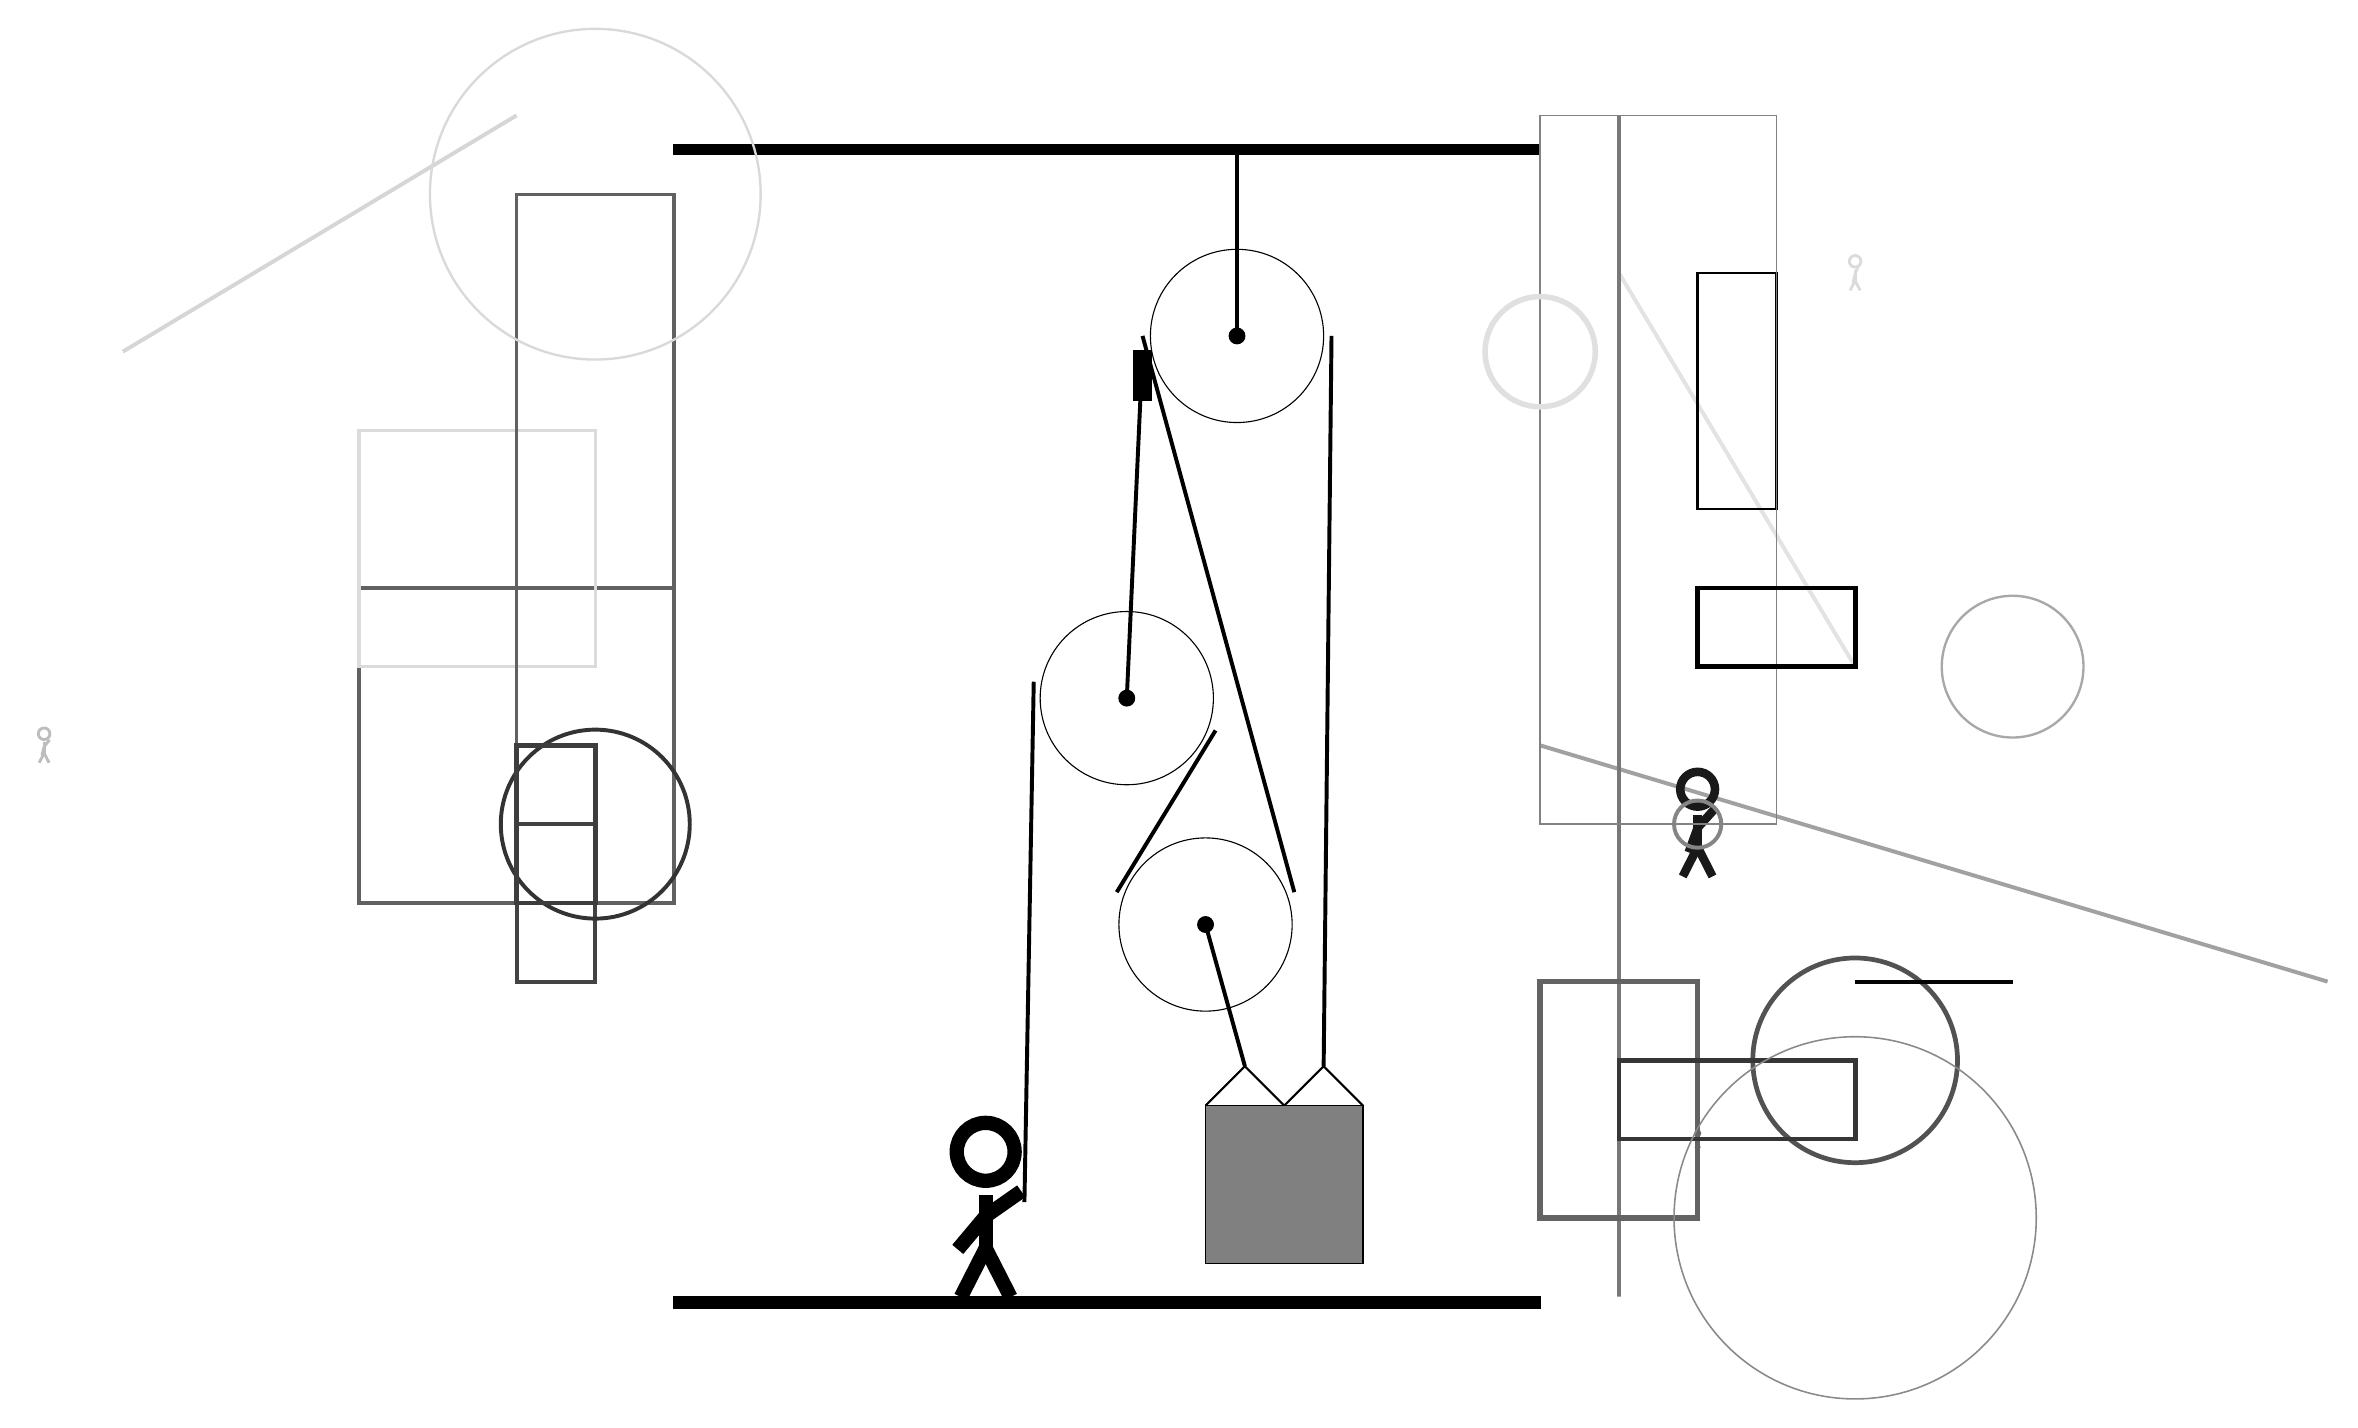
\begin{tikzpicture}
			%%%%% START %%%%%
			
			\draw[fill=black] (-6, 11.5) rectangle (5, 11.625);
			
			\draw (-0.25, 4.6) circle (1.1);
			\draw[fill=black] (-0.25, 4.6) circle (0.1);
			
			\draw (0.75, 1.725) circle (1.1);
			\draw[fill=black] (0.75, 1.725) circle (0.1);
			
			\draw (1.15, 9.2) circle (1.1);
			\draw[fill=black] (1.15, 9.2) circle (0.1);
			\draw[very thick] (1.15, 9.2) -- (1.15, 11.5);
			
			\draw[thick]  (0.75, -0.575) -- (1.25, -0.075) -- (1.75, -0.575) -- (2.25, -0.075) -- (2.75, -0.575);
			\draw[fill=black!50] (0.75, -0.575) rectangle (2.75, -2.575);
			
			\draw[line width=0.5mm, color=black!37](5, 4) -- (15, 1);
			
			\draw [line width=0.6mm, color=black!68](9, 0) circle (1.3);
			\node[line width=0.3mm, color=black!58] at (7, -1) {\Strichmaxerl[1][83][73]};
			\node[line width=0.2mm, color=black!90] at (7, 3) {\Strichmaxerl[6][70][48]};
			\draw[line width=0.5mm, color=black!11](9, 5) -- (6, 10);
			
			\draw[line width=0.5mm, color=black!74] (-8, 1) rectangle (-7, 3);
			\draw[line width=0.3mm, color=black!100] (7, 7) rectangle (8, 10);
			\draw[line width=0.5mm, color=black!62] (-6, 6) rectangle (-10, 2);
			\node[line width=0.7mm, color=black!26] at (-14, 4) {\Strichmaxerl[2][76][51]};
			\draw[line width=0.5mm, color=black!53] (6, 12) rectangle (6, -3);
			\draw[line width=0.5mm, color=black!16](-8, 12) -- (-13, 9);
			\draw [line width=0.3mm, color=black!34](11, 5) circle (0.9);
			\draw[line width=0.4mm, color=black!14] (-7, 8) rectangle (-10, 5);
			
			\draw[line width=0.4mm, color=black!62] (-8, 2) rectangle (-6, 11);
			\draw[line width=0.2mm, color=black!49] (5, 3) rectangle (8, 12);
			\draw[line width=0.7mm, color=black!61] (5, 1) rectangle (7, -2);
			\draw [line width=0.7mm, color=black!12](5, 9) circle (0.7);
			\draw [line width=0.5mm, color=black!48](7, 3) circle (0.3);
			\draw[line width=0.5mm, color=black!99](9, 1) -- (11, 1);
			\draw [line width=0.5mm, color=black!80](-7, 3) circle (1.2);
			\draw[line width=0.6mm, color=black!79] (6, 0) rectangle (9, -1);
			
			\node[line width=0.6mm, color=black!14] at (9, 10) {\Strichmaxerl[2][76][70]};
			\draw [line width=0.2mm, color=black!46](9, -2) circle (2.3);
			\draw [line width=0.3mm, color=black!15](-7, 11) circle (2.1);
			\draw[line width=0.6mm, color=black!76] (-8, 2) rectangle (-7, 4);
			
			\draw[line width=0.6mm, color=black!100] (7, 6) rectangle (9, 5);
			
			\draw[line width=0.5mm] (-0.25, 4.6) -- (-0.05, 9.0);
			\draw[line width=0.5mm, fill=black](-0.15, 8.4) rectangle (0.05, 9.0);
			\draw[line width=0.5mm] (-1.55, -1.8) -- (-1.4318, 4.8083);
			\centerarc[line width=0.5mm](-0.25, 4.6)(-20:170:1.2000000000000002);
			\draw[line width=0.5mm] (0.8776, 4.1896) -- (-0.3776, 2.1354);
			\centerarc[line width=0.5mm](0.75, 1.725)(160:380:1.2000000000000002);
			\draw[line width=0.5mm] (1.8776, 2.1354) -- (-0.05, 9.2);
			\draw[line width=0.5mm](0.75, 1.725) -- (1.25, -0.075);
			\centerarc[line width=0.5mm](1.15, 9.2)(0:180:1.2000000000000002);
			\draw[line width=0.5mm] (2.35, 9.2) -- (2.25, -0.075);
			
			\node at (-2, -1.9) {\Strichmaxerl[10][50][35]};
			
			\draw[fill=black] (-6, -3) rectangle (5, -3.15);
			
			%%%%% END %%%%%
		\end{tikzpicture}
	\end{figure}	
\end{document}